Depending on the application domain, distinct architectural patterns exist that define areas of responsibility that are used to group together software components. Choosing an architectural pattern that fits the application domain can help to organise code, reduce complexity and leverage the experience of developers that have solved similar problems in the past.

\subsection{MVC}
Since the 1970s the Model View Controller (MVC) pattern is the standard software design pattern for applications that present the user with a graphical user interface. It was developed out of a need for modularity, to encapsulate responsibility of specific concepts to separate software modules. MVC identifies three main components that program code should be grouped into, namely\cite{walther_2016}:

\begin{itemize}[label={}]

\item \textbf{Model}: The representation of some object of knowledge, encapsulates code managing the associated data and behaviour ( business-logic ).
\item \textbf{View}: The visual representation of the model. The view can feature or hide aspects of the model and thus act as a presentation filter. The view observes the model for changes and updates the presentation accordingly.
\item \textbf{Controller}: The controller allows the user to interact with the model. It allows the user to trigger behaviours implemented in the Model.

\end{itemize}

In the classic MVC pattern the model does not "know" about the view or the controller. And the controller does not effect the view. Instead, both the view and controller monitor the model using an observer mechanism and synchronise themselves when updates to the model occur.

\begin{figure}[H]
    \centering
    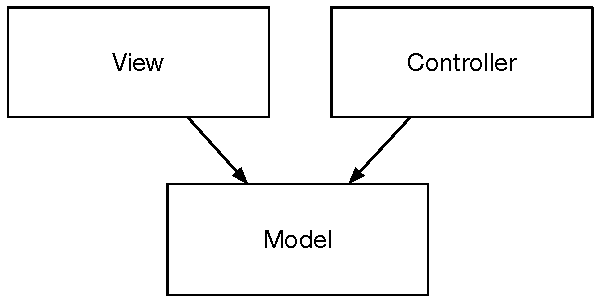
\includegraphics[height=5cm,keepaspectratio]{assets/concept/mvc_1.pdf}
    \caption{Classic MVC}
    \label{fig:mvc_1}
\end{figure}

\subsection{Modern MVC}

Modern MVC has evolved from being a software design pattern which handles components of an application to an architectural design pattern that defines the structure of an application itself. It is similar to a Layer Architecture where each layer interacts directly only with the next layer directly above or below \cite{patterns}. The division of responsibilities is slightly different from the typical presentation,, domain, and data layer definitions.

Most modern web frameworks such as Ruby on Rails, Symfony or the iOS environment refer to themselves as MVC based frameworks. The modern MVC concept has changed slightly. The component definitions are the same, but some responsibilities have shifted. Modern MVC strictly separates the model from the view. All modern frameworks state that the view should have as little logic as possible. Any logic implemented in the view should only be relevant to presentation. The view components should not directly reference the model components\cite{apple_MVC}\cite{symfony_MVC}.


\begin{figure}[H]
    \centering
    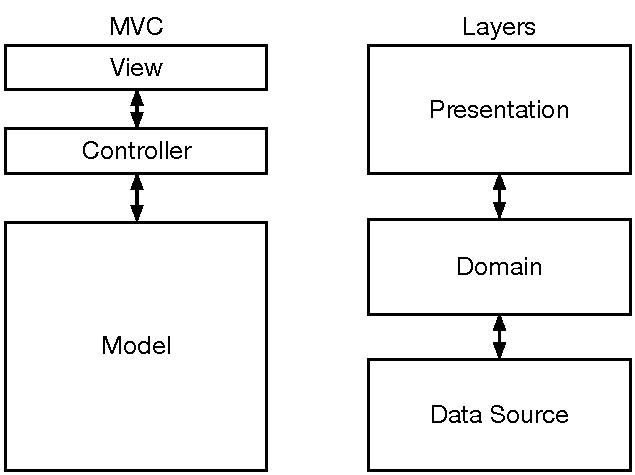
\includegraphics[height=5cm,keepaspectratio]{assets/concept/mvc_2.pdf}
    \caption{Modern MVC vs 3-Layered Architecture}
    \label{fig:mvc_2}
\end{figure}

This division of responsibility has the added benefit of increased testability. GUIs are difficult to test, by removing as much logic as possible from the user interface there is less necessity to test it. The controller and model components can more easily be tested in isolation using normal unit tests\cite{mvp_testing}.

\subsection{MVC Derivatives}

Many MVC derivatives exist. The main differences are where the division of responsibility is made and how it is labeled. MVVM defines a view model instead of a controller. The view model acts as a facade around the model and introduces a data binder element that is responsible for keeping the view and view model synchronised. The MVT, calls the view a template and the controller a view. The slight difference is that the template is basically a static file, with no logic, and placeholders for the data. The Django web framework uses MVT terminology, but there is little difference to the other MVC derivatives such as MVP ( model view presenter ). The AngularJS web framework attempts to end the discussion of which design to follow by labelling itself a MVW ( Model View Whatever ) framework\cite{mvw}.

\begin{figure}[H]
    \centering
    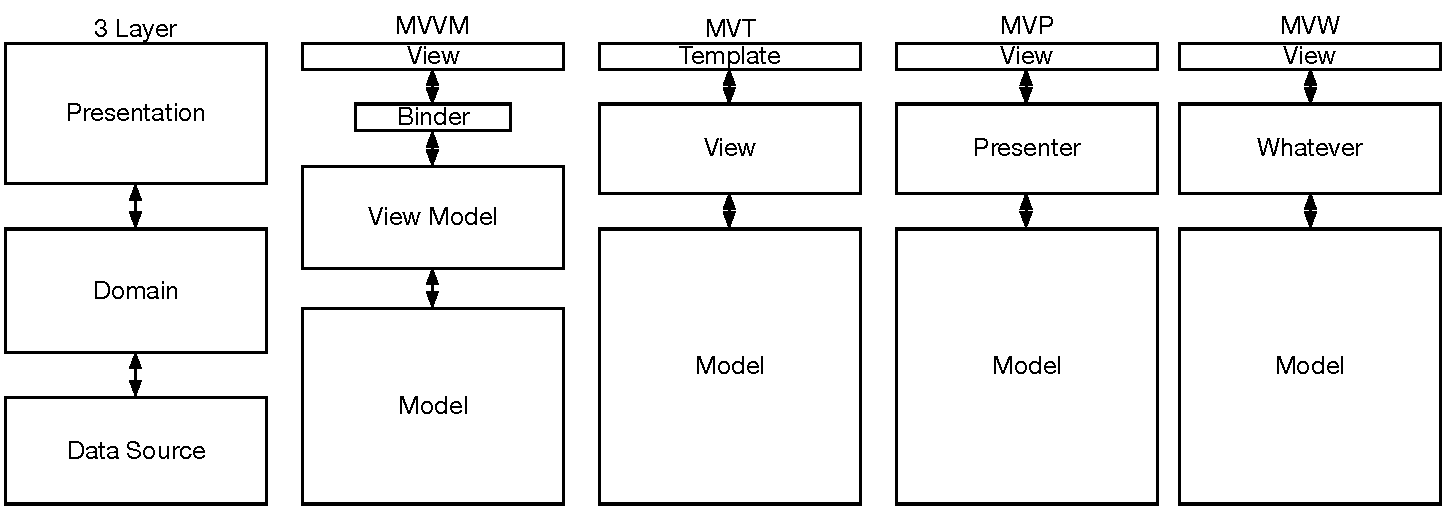
\includegraphics[width=\textwidth,keepaspectratio]{assets/concept/mvc_3.pdf}
    \caption{MVC Derivatives in relation to 3-Tier Layer}
    \label{fig:mvc_alt}
\end{figure}





